% !TeX root = ../main.tex
% Add the above to each chapter to make compiling the PDF easier in some editors.

\chapter{Methodology}\label{chapter:methodology}

\section{Selection Criteria}
The core aim of this research study involves examining and evaluating
various publicly available deepfake detection tools. It becomes imperative
to establish a well-defined set of selection criteria for these tools.
Selecting the right criteria is essential not just for representing a variety
of detection methods, but also for making a fair comparison between the tools.
The objective is to ensure that the evaluated tools are comprehensive,
encompassing the nuances of accessibility, ease of use, limitations, variety
in detection methods, and documentation. A detailed description of the selection
criterias is given in~\autoref{tab:selection_criteria}.

\begin{table}[htpb]
	\caption{Selection Criteria}\label{tab:selection_criteria}
	\centering
	\small
	\begin{tabularx}{\textwidth}{l X}
		\toprule
		\textbf{Selection Criteria} & \textbf{Description}                       \\
		\midrule
		Ease of use and Limitations & The tool's user-friendliness is determined
		by the simplicity of its installation process and its operational
		requirements. Is it a straightforward drag-and-drop mechanism, or does
		it demand an integrated development environment (\ac{IDE}) and
		specialized packages? Additionally, any constraints, such
		as file size limits or video duration caps, play a role in its overall
		user-friendliness.                                                       \\
		\addlinespace
		Accessibility               & Only publicly accessible tools were taken
		into account, promoting the accessibility of deepfake detection and
		ensuring that a wide spectrum of users, from the general public to
		specialists, can utilize the tools. The cost factor is another crucial
		aspect of accessibility; tools that are freely available or open
		source often garner a larger user base compared to proprietary or paid
		solutions. Whether the tools are available through a simple browser
		interface or require local installation can greatly influence
		accessibility. Additionally, while some advanced tools might demand
		powerful GPU setups, the most accessible ones should be usable on
		standard hardware configurations or offer cloud-based solutions, like
		Google Colab, to bypass local hardware limitations.                      \\
		\addlinespace
		Support and Documentation   & Robust documentation and active support,
		be it community or developer-driven, are crucial. Comprehensive support
		ensures that users can fully utilize tool features, troubleshoot issues,
		and gain deeper insights into the tool's workings.                       \\
		\addlinespace
		Dataset choice              & The datasets a tool is compatible with or
		recommends can reflect its versatility and potential applications.
		Tools that can adapt to various datasets or come with robust recommended
		datasets are in a favorable position to tackle countless deepfake
		challenges.                                                              \\
		\bottomrule
	\end{tabularx}
\end{table}

\section{Evaluation Metrics}
After careful selection of the tools based on the prescribed criteria, it became
imperative to systematically evaluate them to ensure their, accuracy
and efficiency. This evaluation isn't just about how these tools perform; it's
about understanding their strengths and potential weaknesses.

Each tool has a unique set of features and algorithms that drive its functionality.
However, to compare them on a fair level and to ensure a comprehensive
assessment, a standard set of evaluation metrics is employed. These metrics serve
as a guiding light, illuminating the capabilities of each tool in terms of
detecting deepfakes. The evaluation metrics employed in this study are provided in~\autoref{tab:evaluation_metrics}.

\begin{table}[htpb]
	\caption{Evaluation Metrics}\label{tab:evaluation_metrics}
	\centering
	\small
	\begin{tabularx}{\textwidth}{l X}
		\toprule
		\textbf{Evaluation Metrics}     & \textbf{Description}                                 \\
		\midrule
		Processing time and scalability & Measures the time taken by the tool to detect
		deepfakes in a given input. It also evaluates how well the tool performs
		when the size and the number of the input data increases.                              \\
		\addlinespace
		Interpretability                & Assesses how understandable and transparent
		the results or outputs of the tool are. It's crucial for users to comprehend
		why certain detections are made.                                                       \\
		\addlinespace
		Detection Accuracy              & The proportion of true results (both true
		positives and true negatives) in the total dataset. It provides a comprehensive
		measure of the tool's ability to correctly identify both genuine and deepfake content. \\
		\addlinespace
		Precision                       & The proportion of true positive results in the
		total predicted positives (both true and false positives). It measures the tool's capability to avoid false positives,
		ennsuring that genuine content isn't mistakenly flagged.                               \\
		\addlinespace
		Recall                          & Measures the tool's ability to correctly
		identify actual deepfakes out of all genuine deepfakes presented. It calculates the
		number of actual true positives the tool identifies.                                   \\
		\addlinespace
		F1-Score                        & The harmonic mean of Precision and Recall.
		It provides a balance between the two when there's an uneven class distribution.       \\
		\bottomrule
	\end{tabularx}
\end{table}

\section{Datasets}
Datasets are very important when working with deepfakes. They form the backbone of both
the creation and detection of deepfakes. They also help us train models to create or spot
deepfakes. Today, there are many datasets available that focus on both deepfake images
and videos. In~\autoref{fig:sample-deepfakes} a fake sample image of each dataset is provided.

\subsection{FaceForensics++}\label{section:ff++}
FaceForensics++~\footnote{https://github.com/ondyari/FaceForensics} serves as a comprehensive dataset designed for forensic studies. It
comprises 977 videos sourced from YouTube, over 1,000 unique sequences, and an
impressive collection of more than 8,000 Deepfake videos. Originally launched in
2018, the dataset received significant updates in 2019, making it richer and more
diverse. As highlighted by the creators in their 2019 paper~\cite{roessler2019faceforensicspp},
the videos in the dataset were modified using a mix of techniques. This includes two
graphics-driven methods, namely Face2Face and FaceSwap, as well as two methods rooted
in machine learning: DeepFakes and NeuralTextures. A noteworthy feature of these
manipulation methods is their reliance on both source and target video pairs for input.
This makes the dataset a valuable resource for those looking to understand the
nuances and intricacies of different deepfake generation techniques.

\subsection{Deepfake Detection Challenge Dataset}
The \ac{DFDC} dataset emerged from a collaborative initiative hosted on Kaggle~\cite{kaggle2020},
aiming to combat the rise of deceptive deepfake videos. Started in 2019 and ending
with a big competition in 2020, this challenge saw over 2200 teams competing for an
overall prize of one million dollars. This challenge wasn't just about competing.
It was a call for researchers all over the world to create new tools to spot fake
content. The dataset has 104,500 different deepfake videos from 3,426 paid
actors~\cite{dolhansky2020deepfake}. This variety makes it a great tool to test and improve deepfake detection
methods.

\subsection{Face Forensics in the Wild}
The \ac{FFIW}~\footnote{https://github.com/tfzhou/FFIW} dataset offers 10,000 high-quality
manipulated videos. What's unique about it is the automatic manipulation process. This
process is managed by a domain-adversarial quality assessment network, which means creating
this dataset requires less human intervention. This design ensures that the dataset can
be scaled up easily and at a low human cost~\cite{Zhou_2021_CVPR}.

\subsection{OpenForensics}
The OpenForensics~\footnote{https://github.com/ltnghia/openforensics} dataset is tailored for detecting and segmenting multi-face forgeries.
Its version 1.0.0 houses more than 115,000 real-world images, capturing a total of 334,000 human faces.
Each image in the dataset comes with detailed face-related annotations, like the type
of forgery, bounding boxes, segmentation masks, forgery boundaries, and typical facial
landmarks~\cite{ltnghia-ICCV2021}.


\begin{figure}[htbp]
	\centering
	\begin{subfigure}{.45\textwidth}
		\centering
		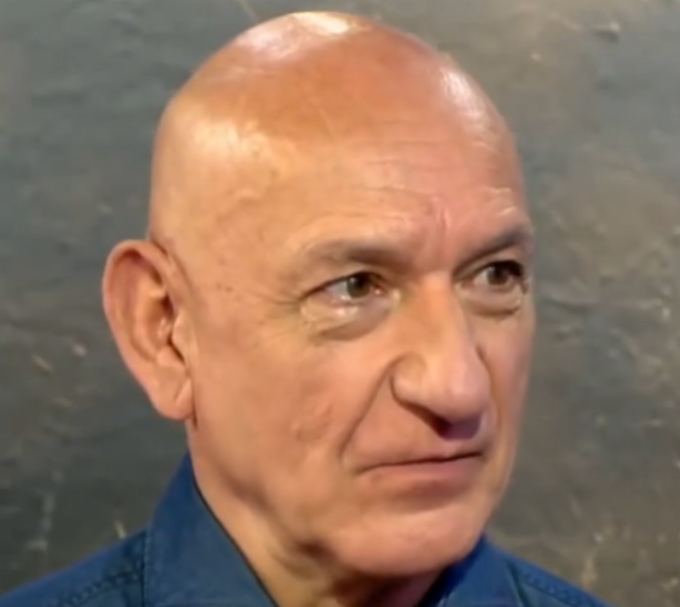
\includegraphics[width=.8\linewidth]{figures/method1}
		\caption{FaceForensics++}\label{fig:sub1}
	\end{subfigure}%
	\hspace{-5mm}
	\begin{subfigure}{.45\textwidth}
		\centering
		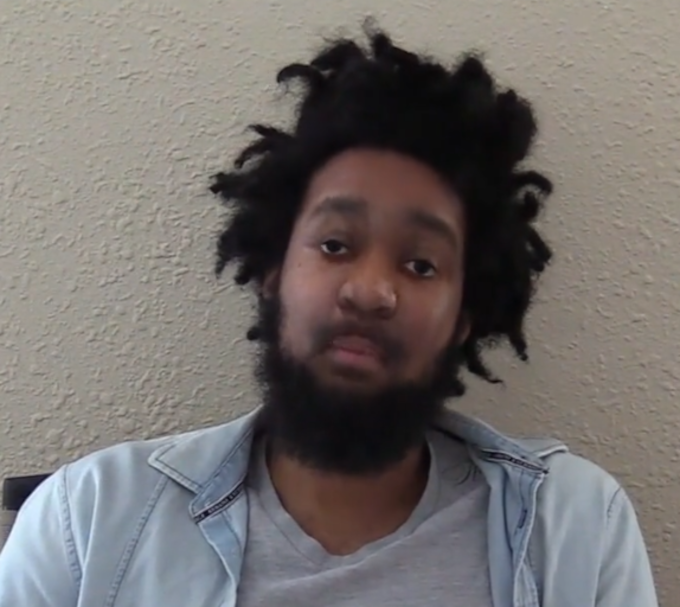
\includegraphics[width=.8\linewidth]{figures/method2}
		\caption{DFDC}\label{fig:sub2}
	\end{subfigure}
	\vspace{5mm} % Adjust the vertical spacing if needed
	\begin{subfigure}{.45\textwidth}
		\centering
		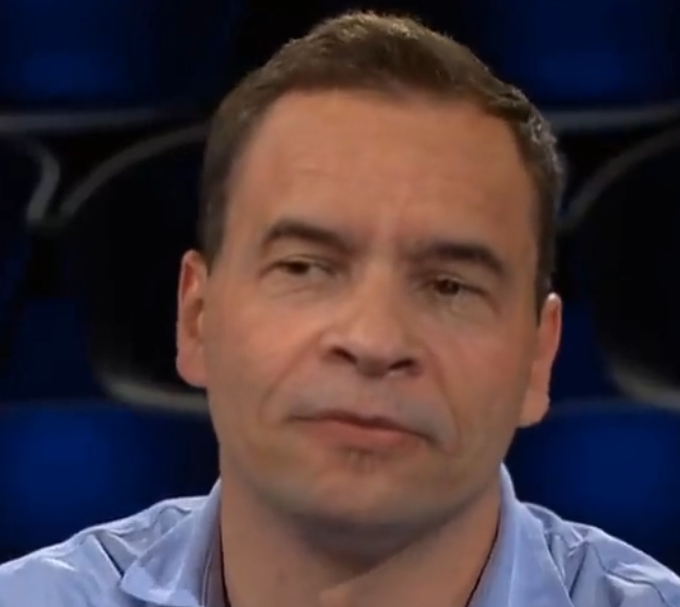
\includegraphics[width=.8\linewidth]{figures/method3}
		\caption{FFIW}\label{fig:sub3}
	\end{subfigure}%
	\hspace{-5mm}
	\begin{subfigure}{.45\textwidth}
		\centering
		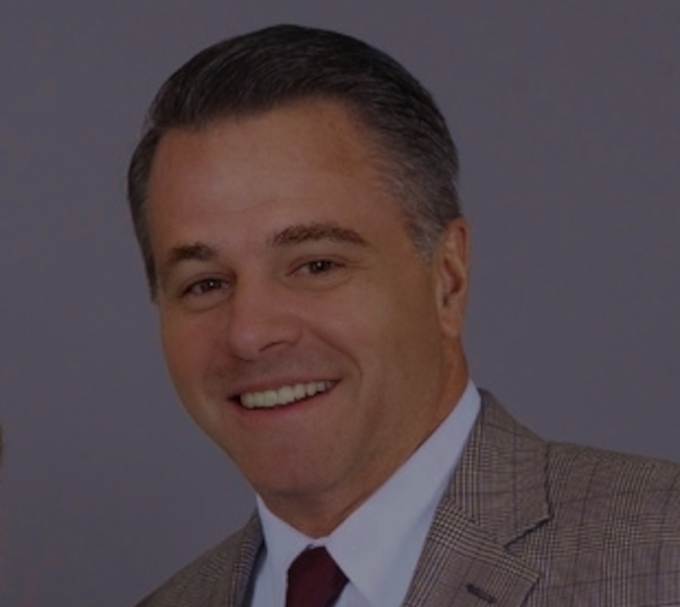
\includegraphics[width=.8\linewidth]{figures/method4}
		\caption{OpenForensics}\label{fig:sub4}
	\end{subfigure}
	\caption{Sample deepfake images taken from FaceForensics++~\cite{roessler2019faceforensicspp},
		DFDC~\cite{dolhansky2020deepfake}, FFIW~\cite{Zhou_2021_CVPR}
		and OpenForensics~\cite{ltnghia-ICCV2021}}\label{fig:sample-deepfakes}
\end{figure}
